% !TeX spellcheck = <none>
\chapter{Sprint 1 – Gestion des utilisateurs et les rôles}
	
\section*{Introduction}
Ce chapitre fait l’objet d’une présentation du deuxième sprint du projet. Ce dernier comporte la gestion des utilisateurs et leurs rôles.

\section[Sprint Backlog]{Sprint Backlog}
Le sprint Backlog permet de faciliter la récupération des tâches et qui fait la mise au point du travail tout en précisant les tâches. Ces dernières contiennent tous les user-stories du Product Backlog.
\subsection[But de sprint]{But de sprint}
La première règle à suivre avant de se lancer dans un sprint, l’équipe SCRUM doit obligatoirement définir le but de ce sprint. Et pour cela, nous devons répondre à une question existentielle: Pourquoi faisons-nous ce sprint?\\
Donc, suite à une conversation entre le Product Owner et l’équipe SCRUM, nous avons conclu que le but de notre premier sprint sera : «Gestion des utilisateurs et leurs rôles».
\subsection[User stories]{User stories}
Après avoir déterminé l'objectif exact du sprint, il est temps de déterminer les user stories que nous voulons y inclure. Lors de la sélection de ces user stories, nous devons garder à l'esprit la priorité de chaque user story que nous avons configurée lorsque nous avons établi notre backlog produit.
\begin{longtable}[c]{|l|l|l|}
	\hline
	\rowcolor[HTML]{C0C0C0} 
	User stories &
	Tâches &
	Complexité\footnotemark{}\\ \hline
	\endhead
	%
	\begin{tabular}[c]{@{}l@{}}En tant qu’un \\ administrateur/admin.\\  habilitations, je souhaite de gérer \\ les utilisateurs de Panoramix\end{tabular} &
	\begin{tabular}[c]{@{}l@{}}Ajouter les interfaces de la gestion\\  des utilisateurs\\ \tabitem Consultation\\ \tabitem Modification\\ \tabitem Suppression\\ \tabitem Création \\ \tabitem Recherche\\ et la logique derrière\end{tabular} &
	1 \\ \hline
	\begin{tabular}[c]{@{}l@{}}En tant qu’un \\ administrateur/admin.\\  habilitations, je souhaite\\  d’importer(ADD) ou supprimer \\ (DEL) des utilisateurs à partir d'un\\ fichier csv\end{tabular} &
	\begin{tabular}[c]{@{}l@{}}Ajouter bouton “importer” dans \\ l’interface de gestion des\\  utilisateurs et la logique derrière \\ en fonction de structure de le \\ fichier csv\end{tabular} &
	2 \\ \hline
	\begin{tabular}[c]{@{}l@{}}En tant qu’un \\ administrateur/admin. \\ habilitations, je souhaite\\ d’exporter les informations des \\ utilisateurs dans un fichier csv\end{tabular} &
	\begin{tabular}[c]{@{}l@{}}Ajouter bouton “exporter” dans\\ l’interface de gestion des \\ utilisateurs et la logique derrière\end{tabular} &
	2 \\ \hline
	\begin{tabular}[c]{@{}l@{}}En tant qu’un administrateur, je \\ souhaite de gérer les rôles\end{tabular} &
	\begin{tabular}[c]{@{}l@{}}Ajouter les interfaces de la gestion\\  des rôles\\ \tabitem Consultation\\ \tabitem Modification\\ \tabitem Suppression\\ \tabitem Création\\ \tabitem Recherche\\ et la logique derrière\end{tabular} &
	1 \\ \hline
	\begin{tabular}[c]{@{}l@{}}En tant qu’un administrateur, je\\  souhaite de gérer les types de rôles\end{tabular} &
	\begin{tabular}[c]{@{}l@{}}Ajouter les interfaces de la gestion \\ des types de rôles\\ \tabitem Consultation des types de rôles.\\ \tabitem Attribution de types au rôle\\ \tabitem Modification de types\\ \tabitem Suppression de l’attribution\\ \tabitem Recherche \\ et la logique derrière\end{tabular} &
	2 \\ \hline
	\begin{tabular}[c]{@{}l@{}}En tant qu’un administrateur, je\\  souhaite d’activer/désactiver le \\ rôles attribué à un utilisateur\end{tabular} &
	\begin{tabular}[c]{@{}l@{}}Ajouter les interfaces de la \\ gestion des rôles\\ \tabitem Consultation\\ \tabitem Modification\\ \tabitem  Recherche\\ et la logique derrière\end{tabular} &
	2 \\ \hline
	\captionsetup{justification=centering}
	\caption{user stories sprint 1}
	\label{tab:user-stories-sprint1}\\
\end{longtable}
\footnotetext{plus faible plus complexe}

\section{Etude et réalisation du sprint 1}
La deuxième partie de notre projet, qui représente le module de gestion des utilisateurs et leurs rôles, nous donne la possibilité d’ajouter la nouvelle population C’Pro.
\subsection{Diagramme de cas d’utilisation global sprint 1}
La figure \ref{fig:usecase-sprint1} décrit le diagramme de cas d’utilisation global du sprint 1.
\begin{figure}[H]
	\centering
	\includegraphics[width=0.7\linewidth]{"img/conception/usecases/sprint 1/usecase-Sprint1"}
	\caption[Diagramme de cas d’utilisation global sprint 1]{Diagramme de cas d’utilisation global sprint 1}
	\label{fig:usecase-sprint1}
\end{figure}
\subsection{Raffinement et description textuelle des diagrammes de cas d’utilisation}
Dans cette section, nous présentons les diagrammes des cas d’utilisation détaillés et leurs descriptions textuelles.
\subsubsection{Cas d’utilisation «Gérer utilisateurs»}
La figure \ref{fig:usecase-gestion-users} décrit le raffinement du cas d’utilisation « Gérer utilisateurs »
\begin{figure}[H]
	\centering
	\includegraphics[width=0.7\linewidth]{"img/conception/usecases/sprint 1/usecase-gestion-users"}
	\caption[Cas d’utilisation «Gérer utilisateurs»]{Cas d’utilisation «Gérer utilisateurs»}
	\label{fig:usecase-gestion-users}
\end{figure}
\myparagraph{Description textuelle du cas d’utilisation «Gérer utilisateurs»}
Le tableau \ref{tab:Description-textuelle-du-cas-utilisation-gerer-utilisateurs} contient la description textuelle du cas d’utilisation« Gérer Utilisateurs»

\begin{table}[H]
	\resizebox{\textwidth}{!}{%
		\begin{tabular}{|l|l|}
			\hline
			\rowcolor[HTML]{C0C0C0} 
			Cas d’utilisation & Gérer utilisateurs                                                                 \\ \hline
			Acteurs           & Administrateur, Administrateur Habilitation                                        \\ \hline
			Résumé            & L’administrateur des habilitations ou l’administrateur peut gérer les utilisateurs \\ \hline
			Pré-condition     & L’acteur doit être authentifié                                                     \\ \hline
			Scénario principal &
			\begin{tabular}[c]{@{}l@{}}Pour gérer les utilisateurs, l’acteur peut :\\ Ajouter un utilisateur\\ Modifier un utilisateur\\ Supprimer un utilisateur\\ Consulter les utilisateurs\\ Import des utilisateurs ou les supprimer en masse en\\ basant sur le champs action ( soit ADD, soit DEL)\\ Exporter les utilisateurs dans un fichier csv\end{tabular} \\ \hline
			Post-condition    & Mettre à jour la liste des utilisateurs                                            \\ \hline
		\end{tabular}%
	}
	\captionsetup{justification=centering}
	\caption{Description textuelle du cas d’utilisation «Gérer utilisateurs»}
	\label{tab:Description-textuelle-du-cas-utilisation-gerer-utilisateurs}
\end{table}

\subsubsection{Cas d’utilisation «Gérer rôles»}
La figure \ref{fig:usecase-gestion-roles-1} illustre le raffinement du cas d’utilisation «Gérer rôles»
\begin{figure}[H]
	\centering
	\includegraphics[width=01\linewidth]{"img/conception/usecases/sprint 1/usecase-gestion-roles-1"}
	\caption[cas d’utilisation «Gérer rôles»]{cas d’utilisation «Gérer rôles»}
	\label{fig:usecase-gestion-roles-1}
\end{figure}
\myparagraph{Description textuelle du cas d’utilisation «Gérer rôles»}
Le tableau \ref{tab:Description-textuelle-du-cas-utilisation-gerer-roles} contient la description textuelle du cas d’utilisation «Gérer rôles».

\begin{table}[H]
	\centering
	\begin{tabular}{|l|l|}
		\hline
		\rowcolor[HTML]{C0C0C0} 
		Cas d’utilisation & Gérer rôles                            \\ \hline
		Acteurs           & Administrateur                         \\ \hline
		Résumé            & L’administrateur peut gérer les rôles  \\ \hline
		Pré-condition     & L'administrateur doit être authentifié \\ \hline
		Scénario principal &
		\begin{tabular}[c]{@{}l@{}}Pour gérer les rôles, l’administrateur peut :\\ Ajouter un rôle\\ Modifier un rôle\\ Supprimer un rôle\\ Consulter les rôles\\ gestion des types de rôles\\ activation des rôles attribué à un utilisateur\end{tabular} \\ \hline
		Post-condition    & Mettre à jour la liste des rôles       \\ \hline
	\end{tabular}
	\captionsetup{justification=centering}
	\caption{Description textuelle du cas d’utilisation «Gérer utilisateurs»}
	\label{tab:Description-textuelle-du-cas-utilisation-gerer-roles}
\end{table}

\section{Conception}
Dans cette partie, nous présentons les différents diagrammes de classes ainsi que de séquence détaillés pour ce sprint.
\subsection{Diagramme de classes}
la figure \ref{fig:classdiag-sprint1} illustre la structure statique du sprint 1 schématisé dans un diagramme de classe globale.
\begin{figure}[H]
	\centering
	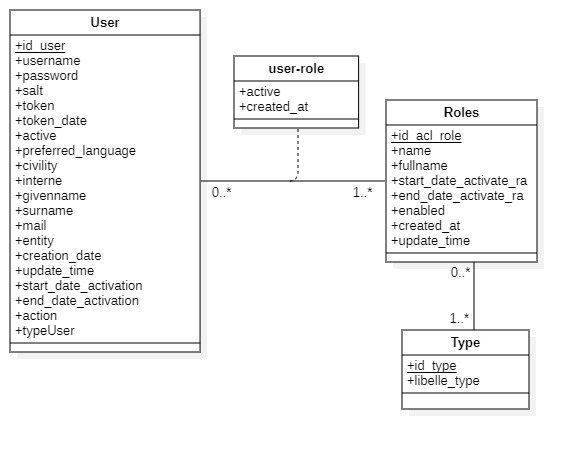
\includegraphics[width=0.7\linewidth]{img/conception/classes/ClassDiag-sprint1}
	\caption[Diagramme de classes de sprint 1]{Diagramme de classes de sprint 1}
	\label{fig:classdiag-sprint1}
\end{figure}
\subsection{diagramme de séquences détaillés}
Nous allons maintenant passer à l’aspect dynamique des opérations représentées dans le diagramme de classe à l’aide des diagrammes de séquences de système et d’objets.
\subsubsection{Quelques diagramme de séquences système de Sprint 1}
Dans cette section, nous présenterons quelques diagrammes de séquences système de sprint 1 tels que : \newpage
\myparagraph{Diagramme de séquences système d’«Ajouter Utilisateur»}
\begin{figure}[H]
	\centering
	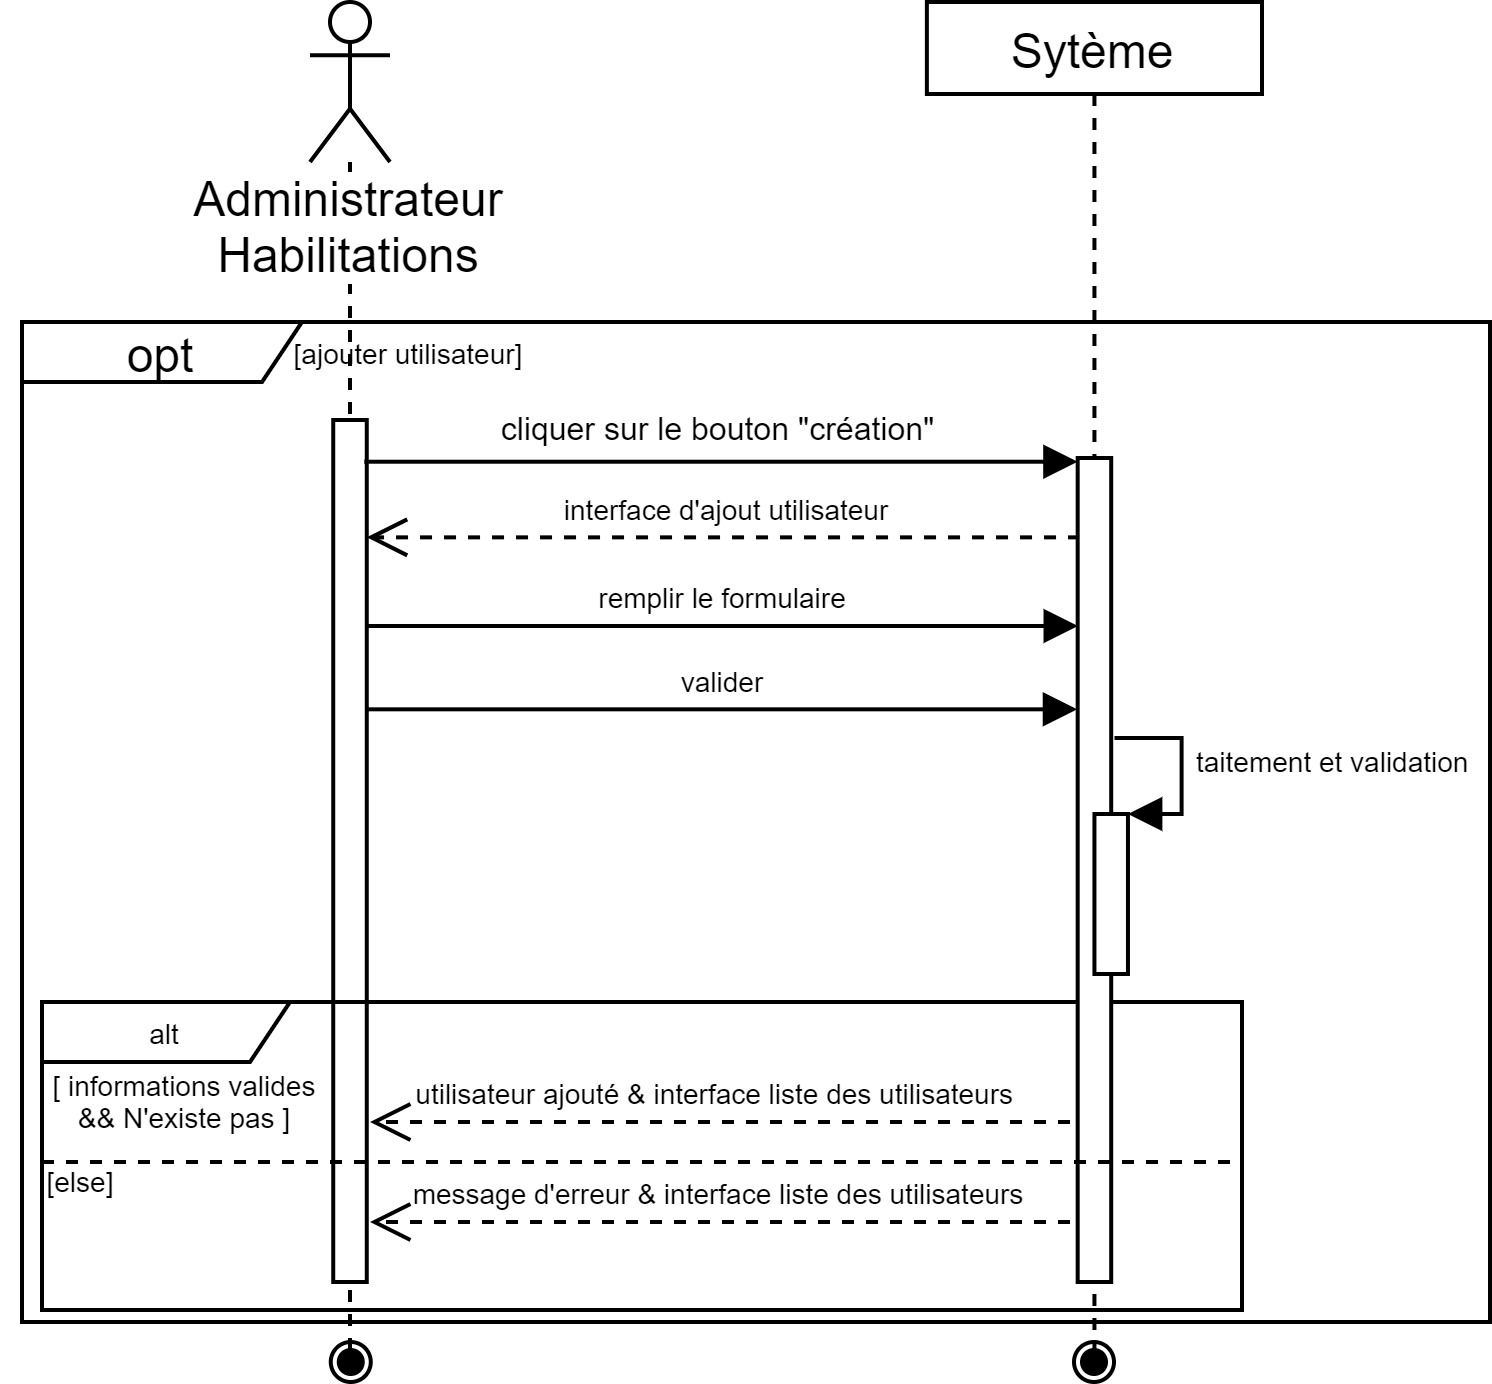
\includegraphics[width=0.65\linewidth]{img/conception/sequences/add-user}
	\caption[Diagramme de séquences système d’ «Ajouter Utilisateur»]{Diagramme de séquences système d’ «Ajouter Utilisateur»}
	\label{fig:add-user}
\end{figure}

\myparagraph{Diagramme de séquences système de «Supprimer Utilisateur»}
\begin{figure}[H]
	\centering
	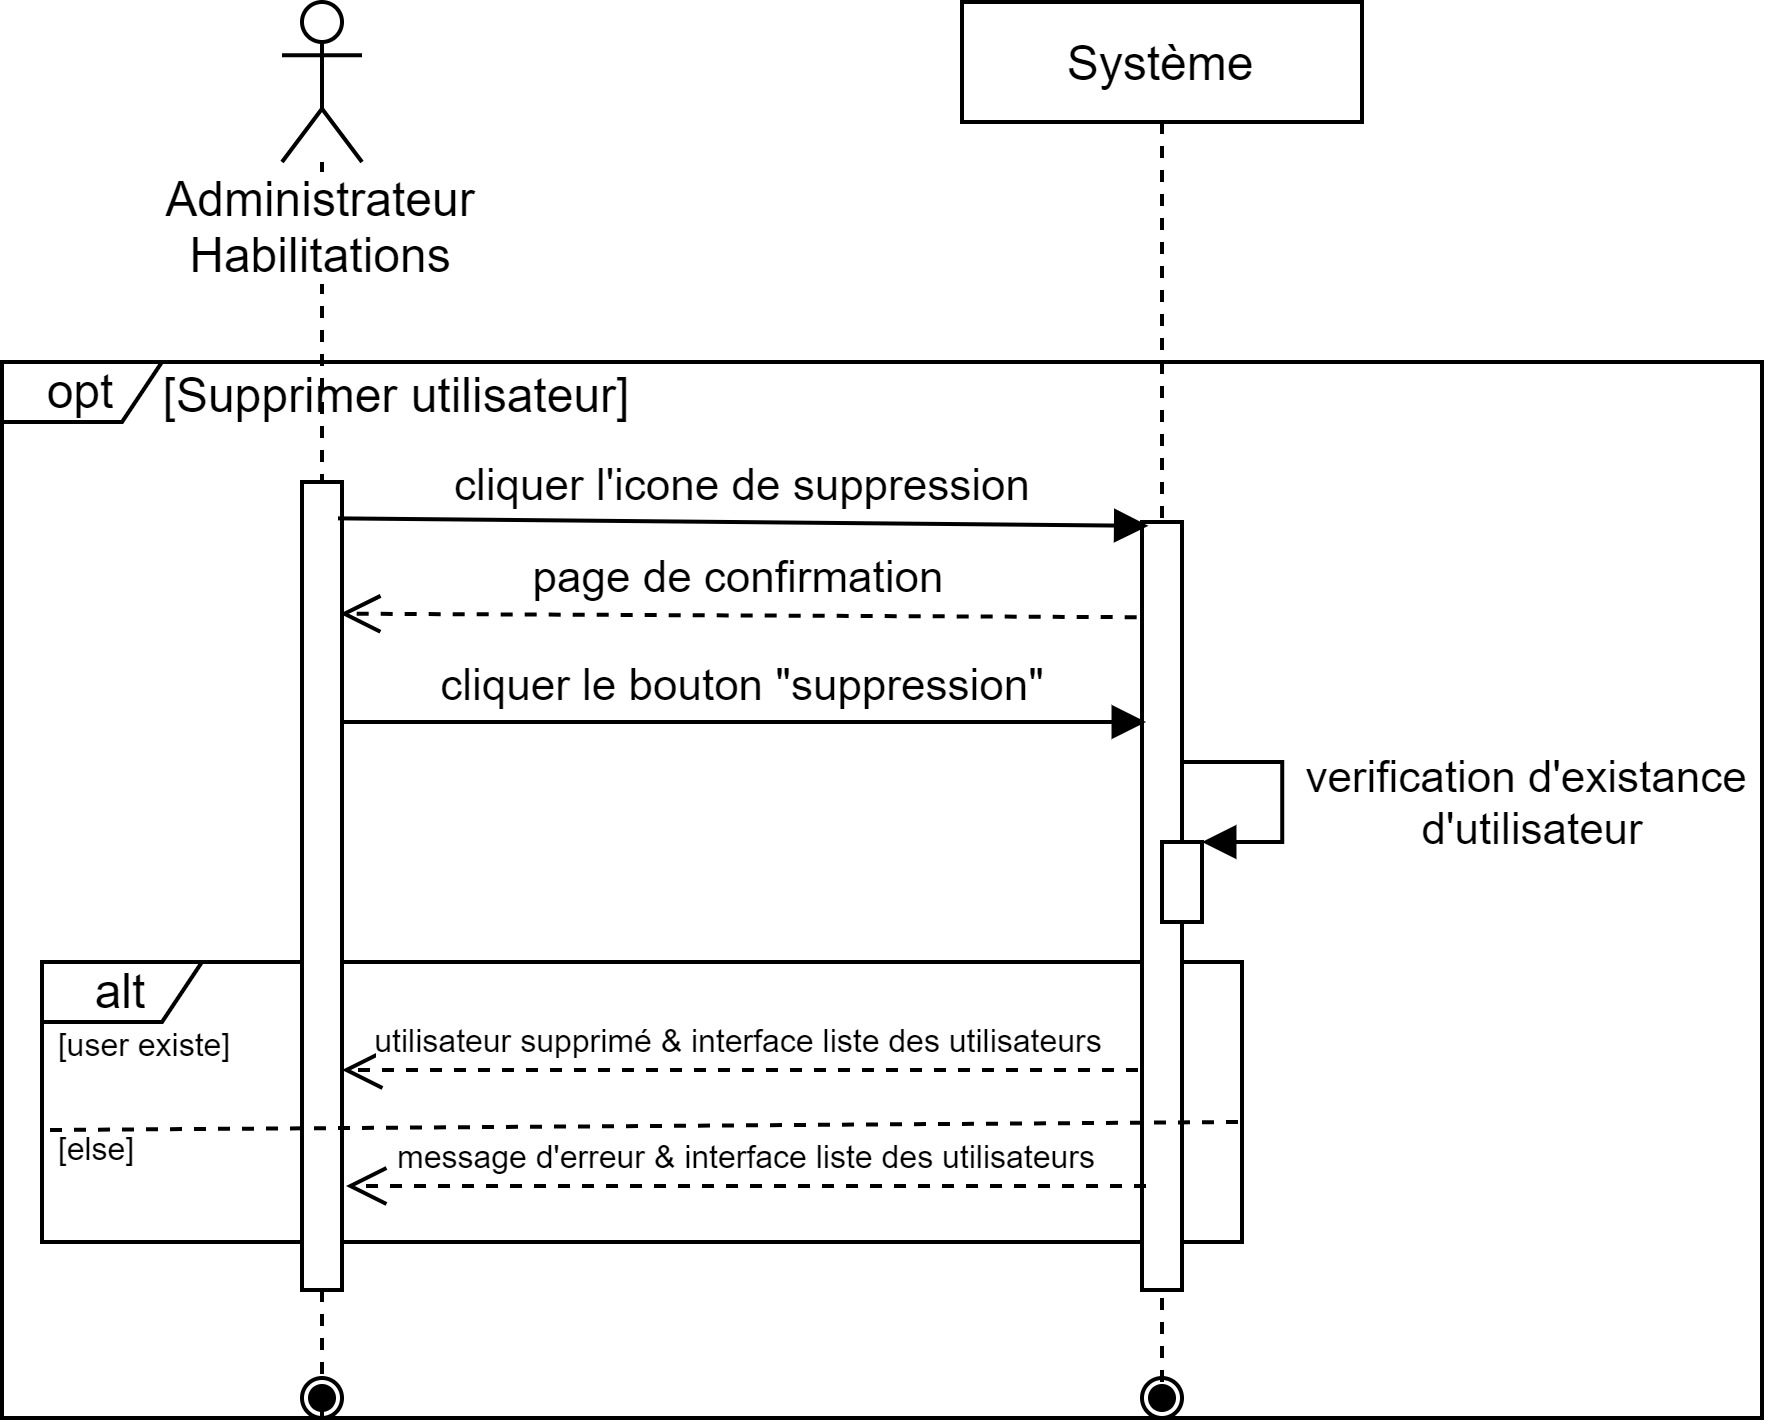
\includegraphics[width=0.65\linewidth]{img/conception/sequences/delete-user}
	\caption[Diagramme de séquences système de «Supprimer Utilisateur»]{Diagramme de séquences système de «Supprimer Utilisateur»}
	\label{fig:delete-user}
\end{figure}

\myparagraph{Diagramme de séquences système d’«Importer Utilisateurs»}
\begin{figure}[H]
	\centering
	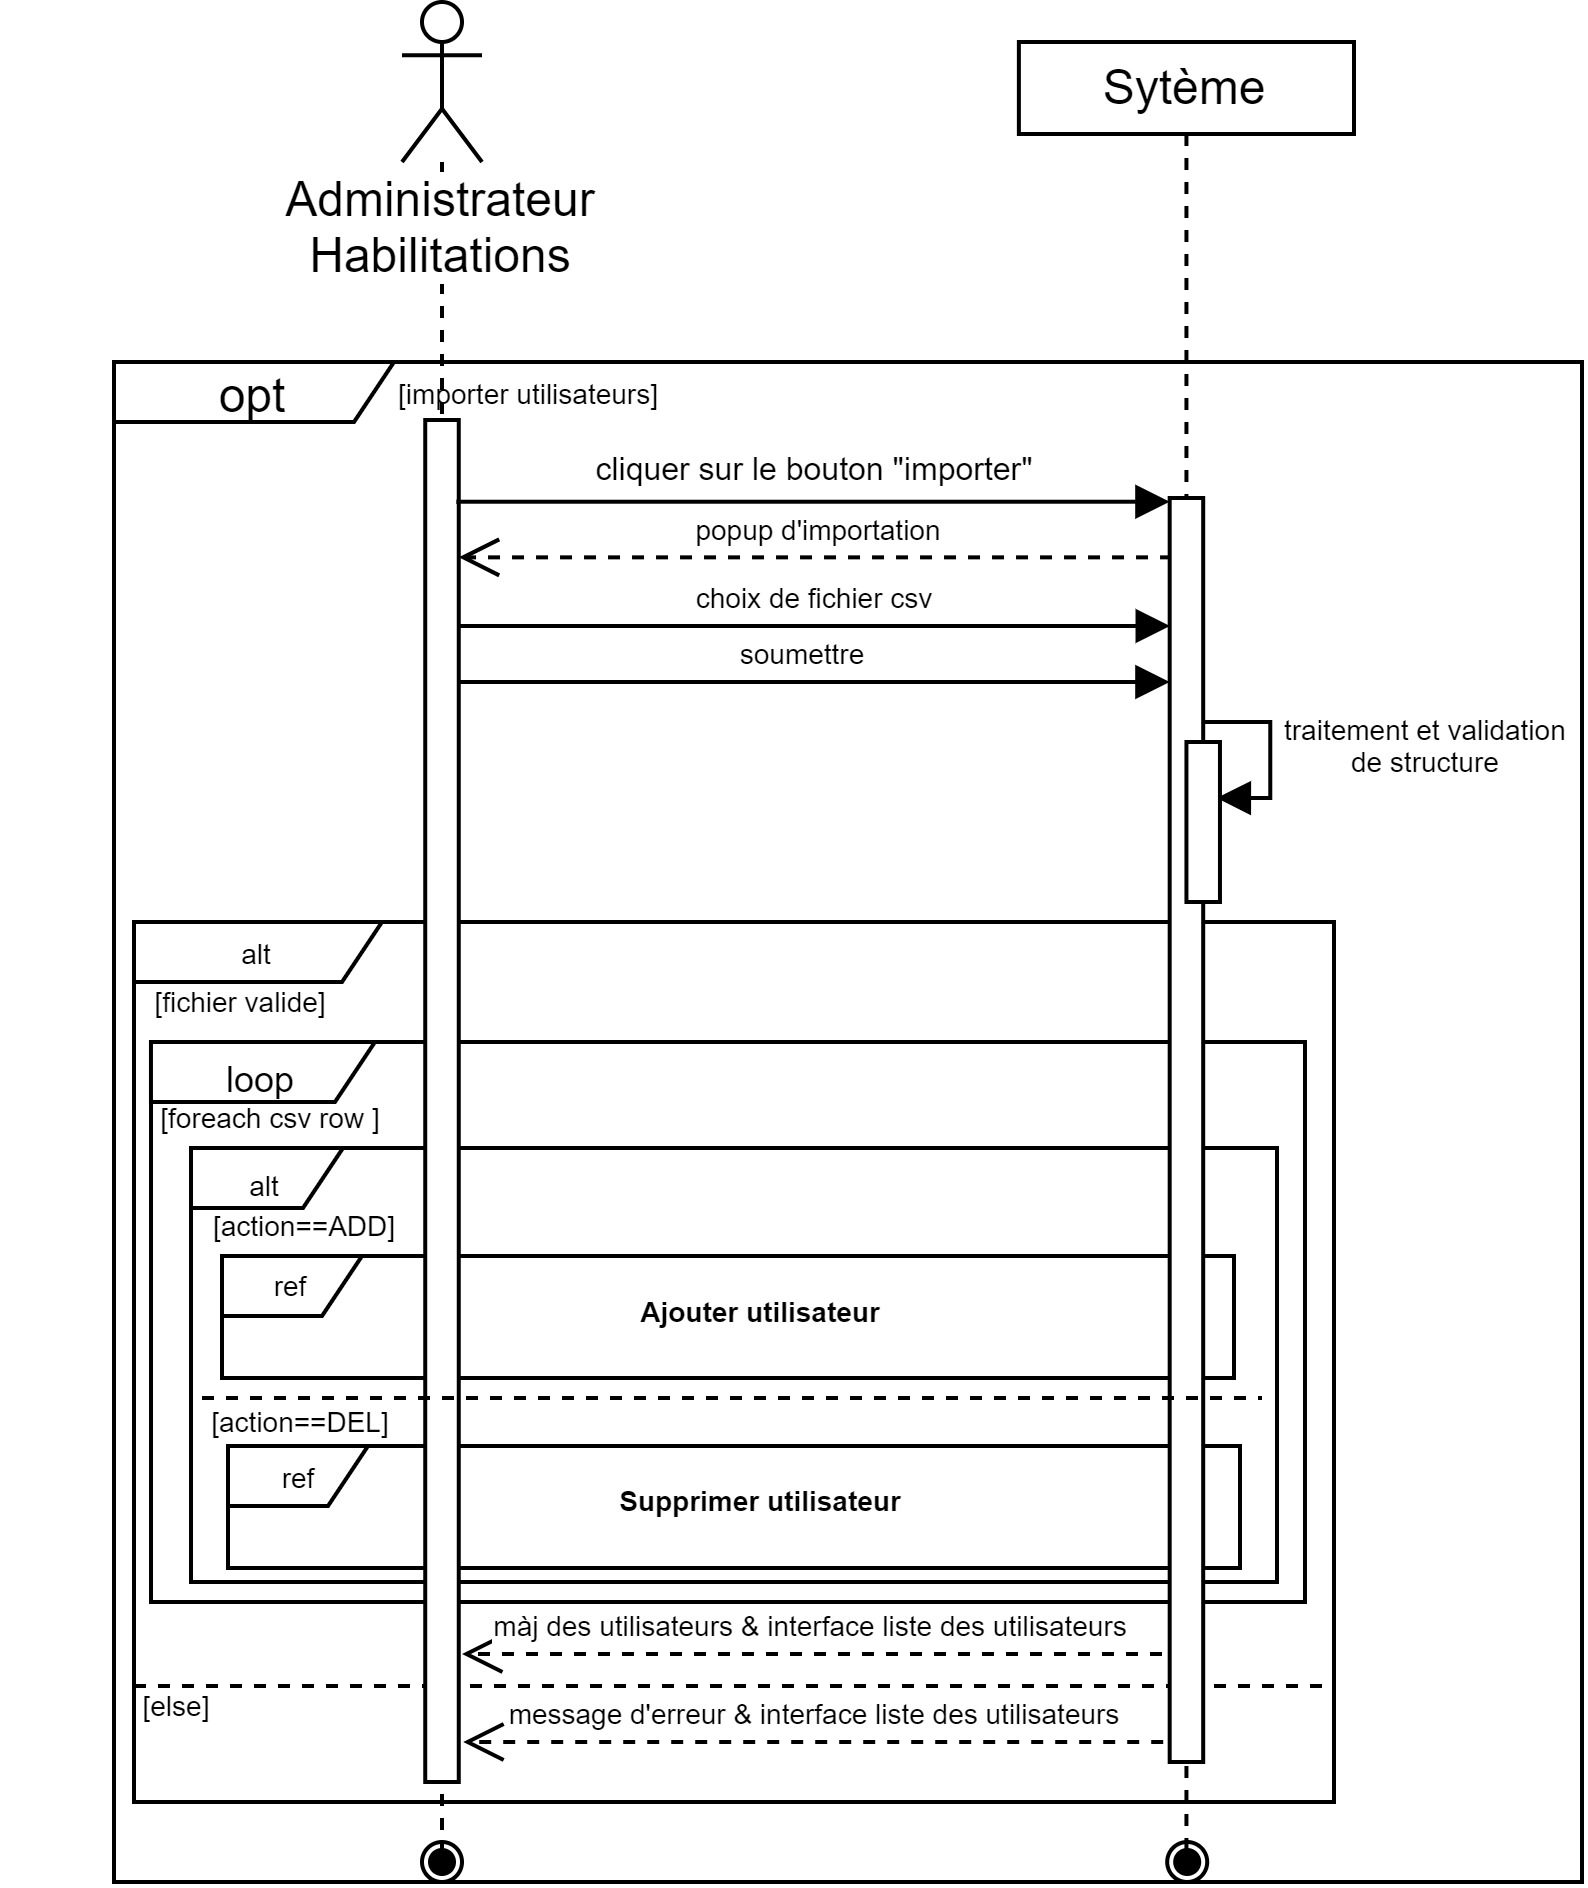
\includegraphics[width=0.65\linewidth]{img/conception/sequences/import}
	\caption[Diagramme de séquences système d’ «Importer Utilisateur»]{Diagramme de séquences système d' «Importer Utilisateurs»}
	\label{fig:import}
\end{figure}

\subsubsection{Diagramme de séquences objets de Sprint 1}
Nous présentons dans ce qui suit quelques diagrammes de séquences objets détaillés du \\sprint 1.
\newpage
\myparagraph{Diagramme de séquences objets d’«Ajouter Utilisateur» }
\begin{figure}[H]
	\centering
	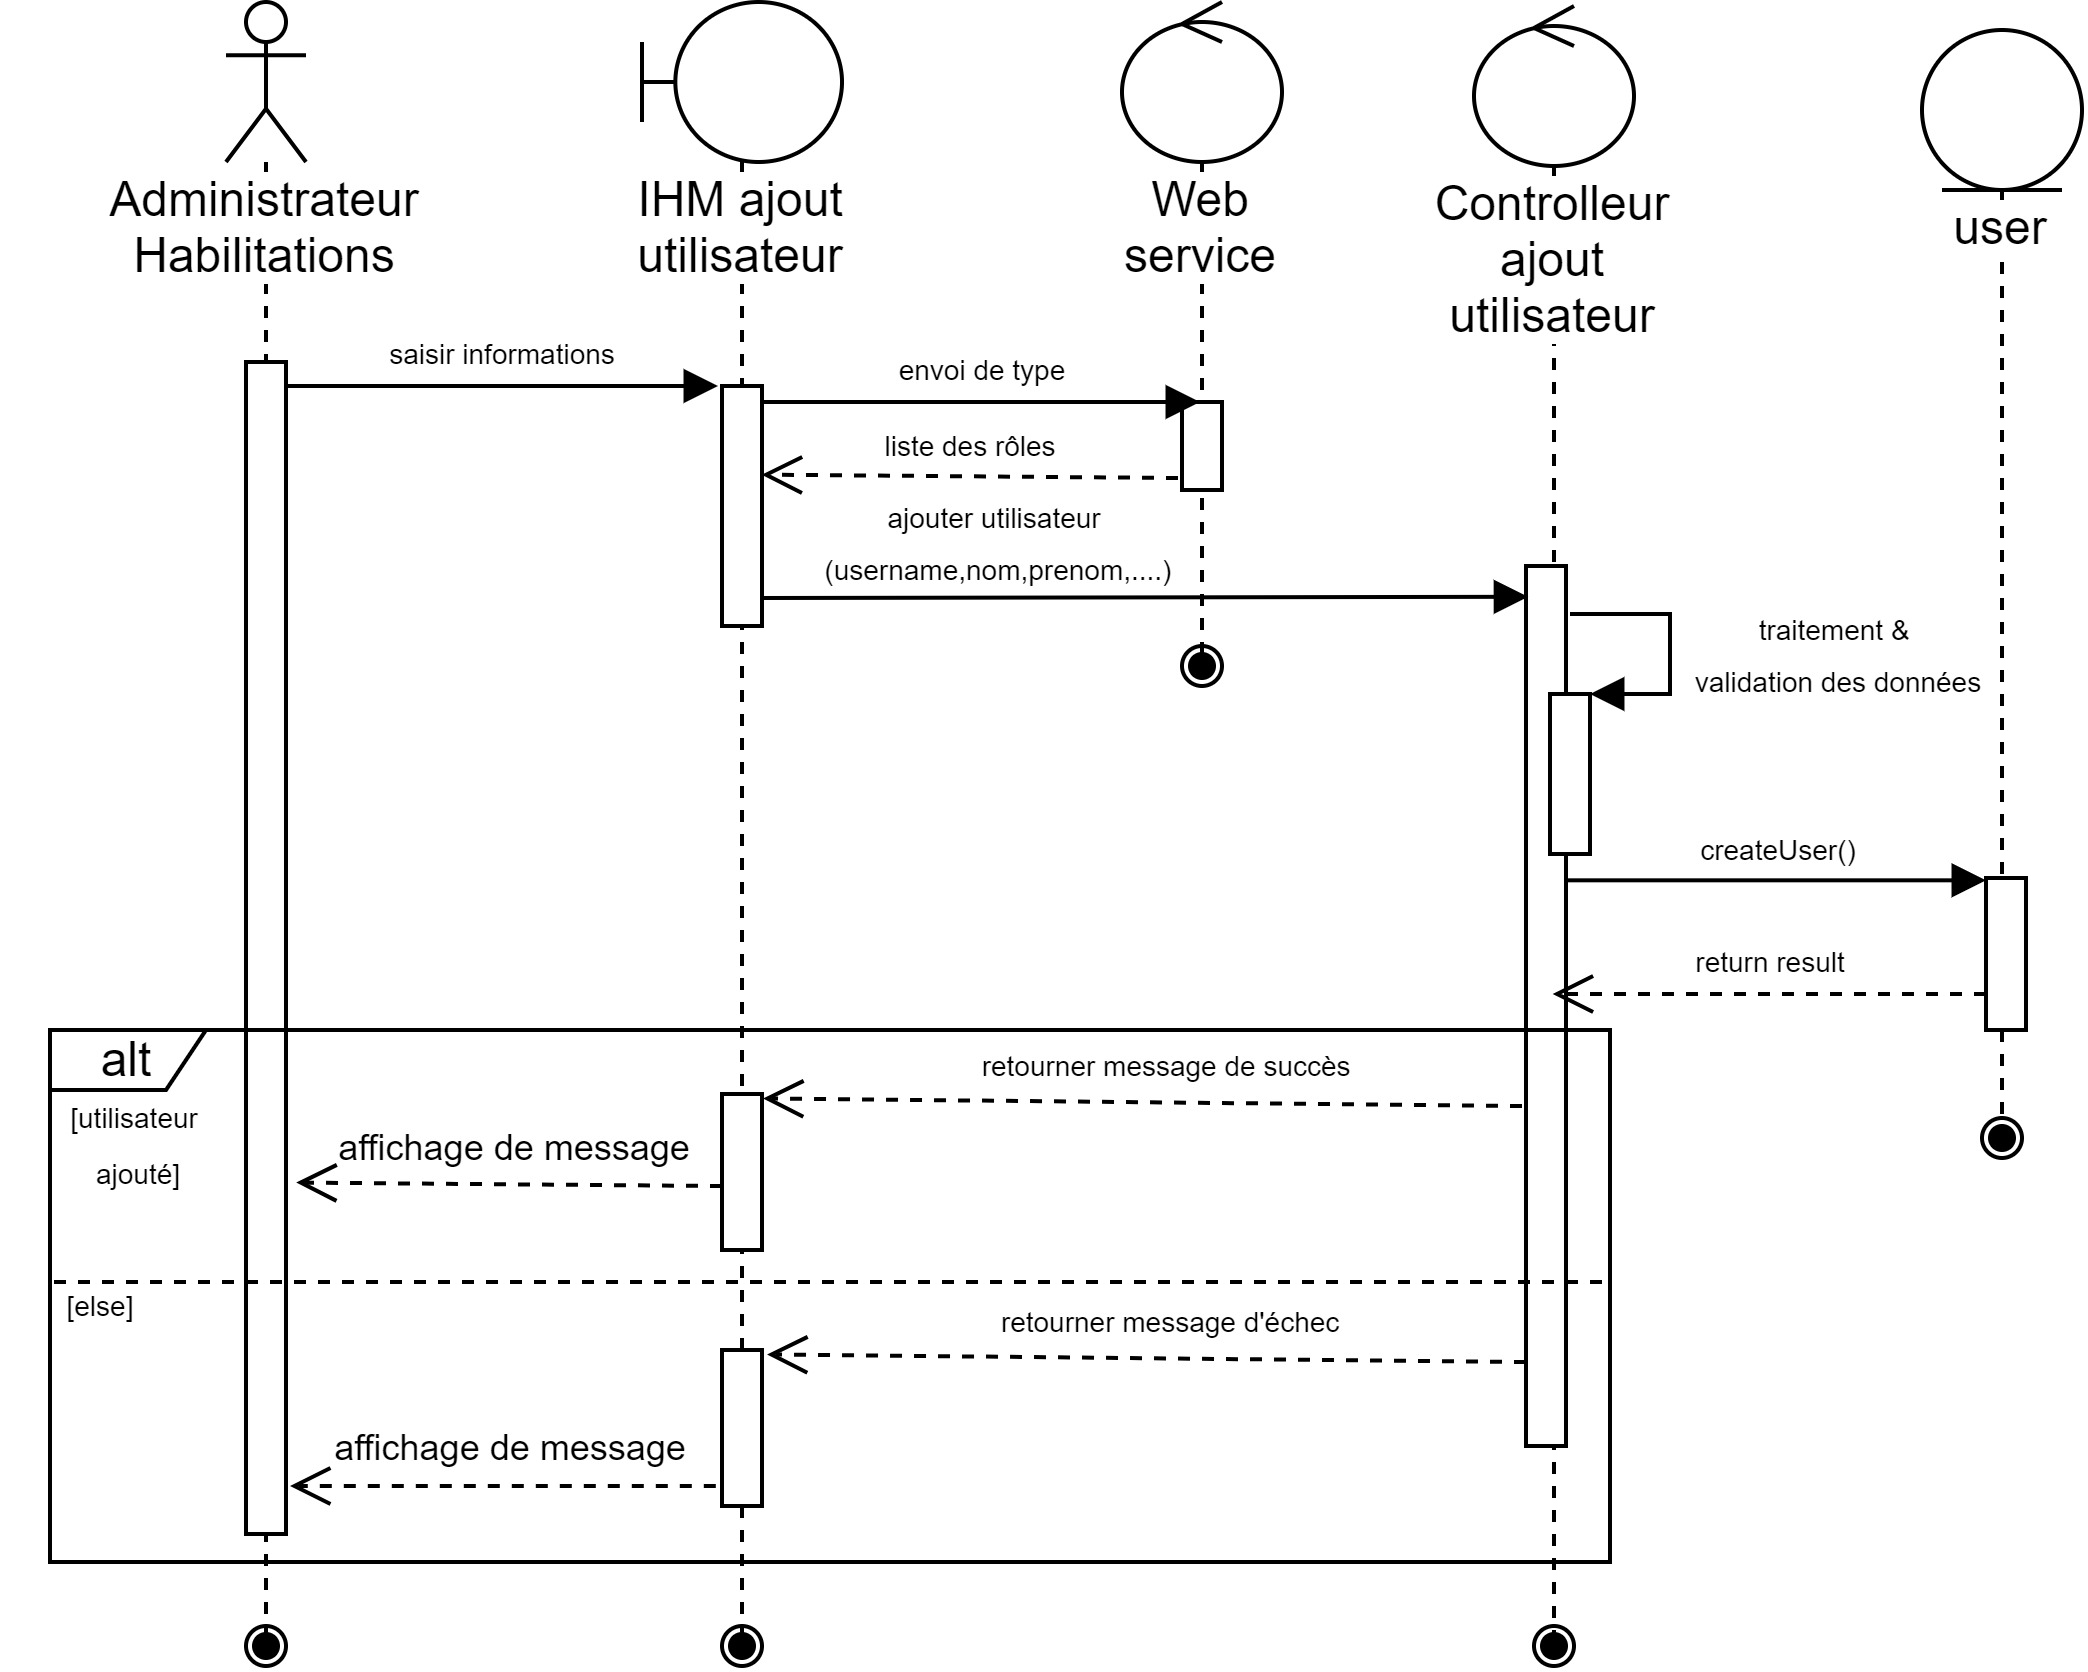
\includegraphics[width=0.75\linewidth]{img/conception/sequences/add-user-obj}
	\caption[Diagramme de séquences objets d’«Ajouter Utilisateur»]{Diagramme de séquences objets d’«Ajouter Utilisateur»}
	\label{fig:add-user-obj}
\end{figure}

\myparagraph{Diagramme de séquences objets de «Supprimer Utilisateur» }
\begin{figure}[H]
	\centering
	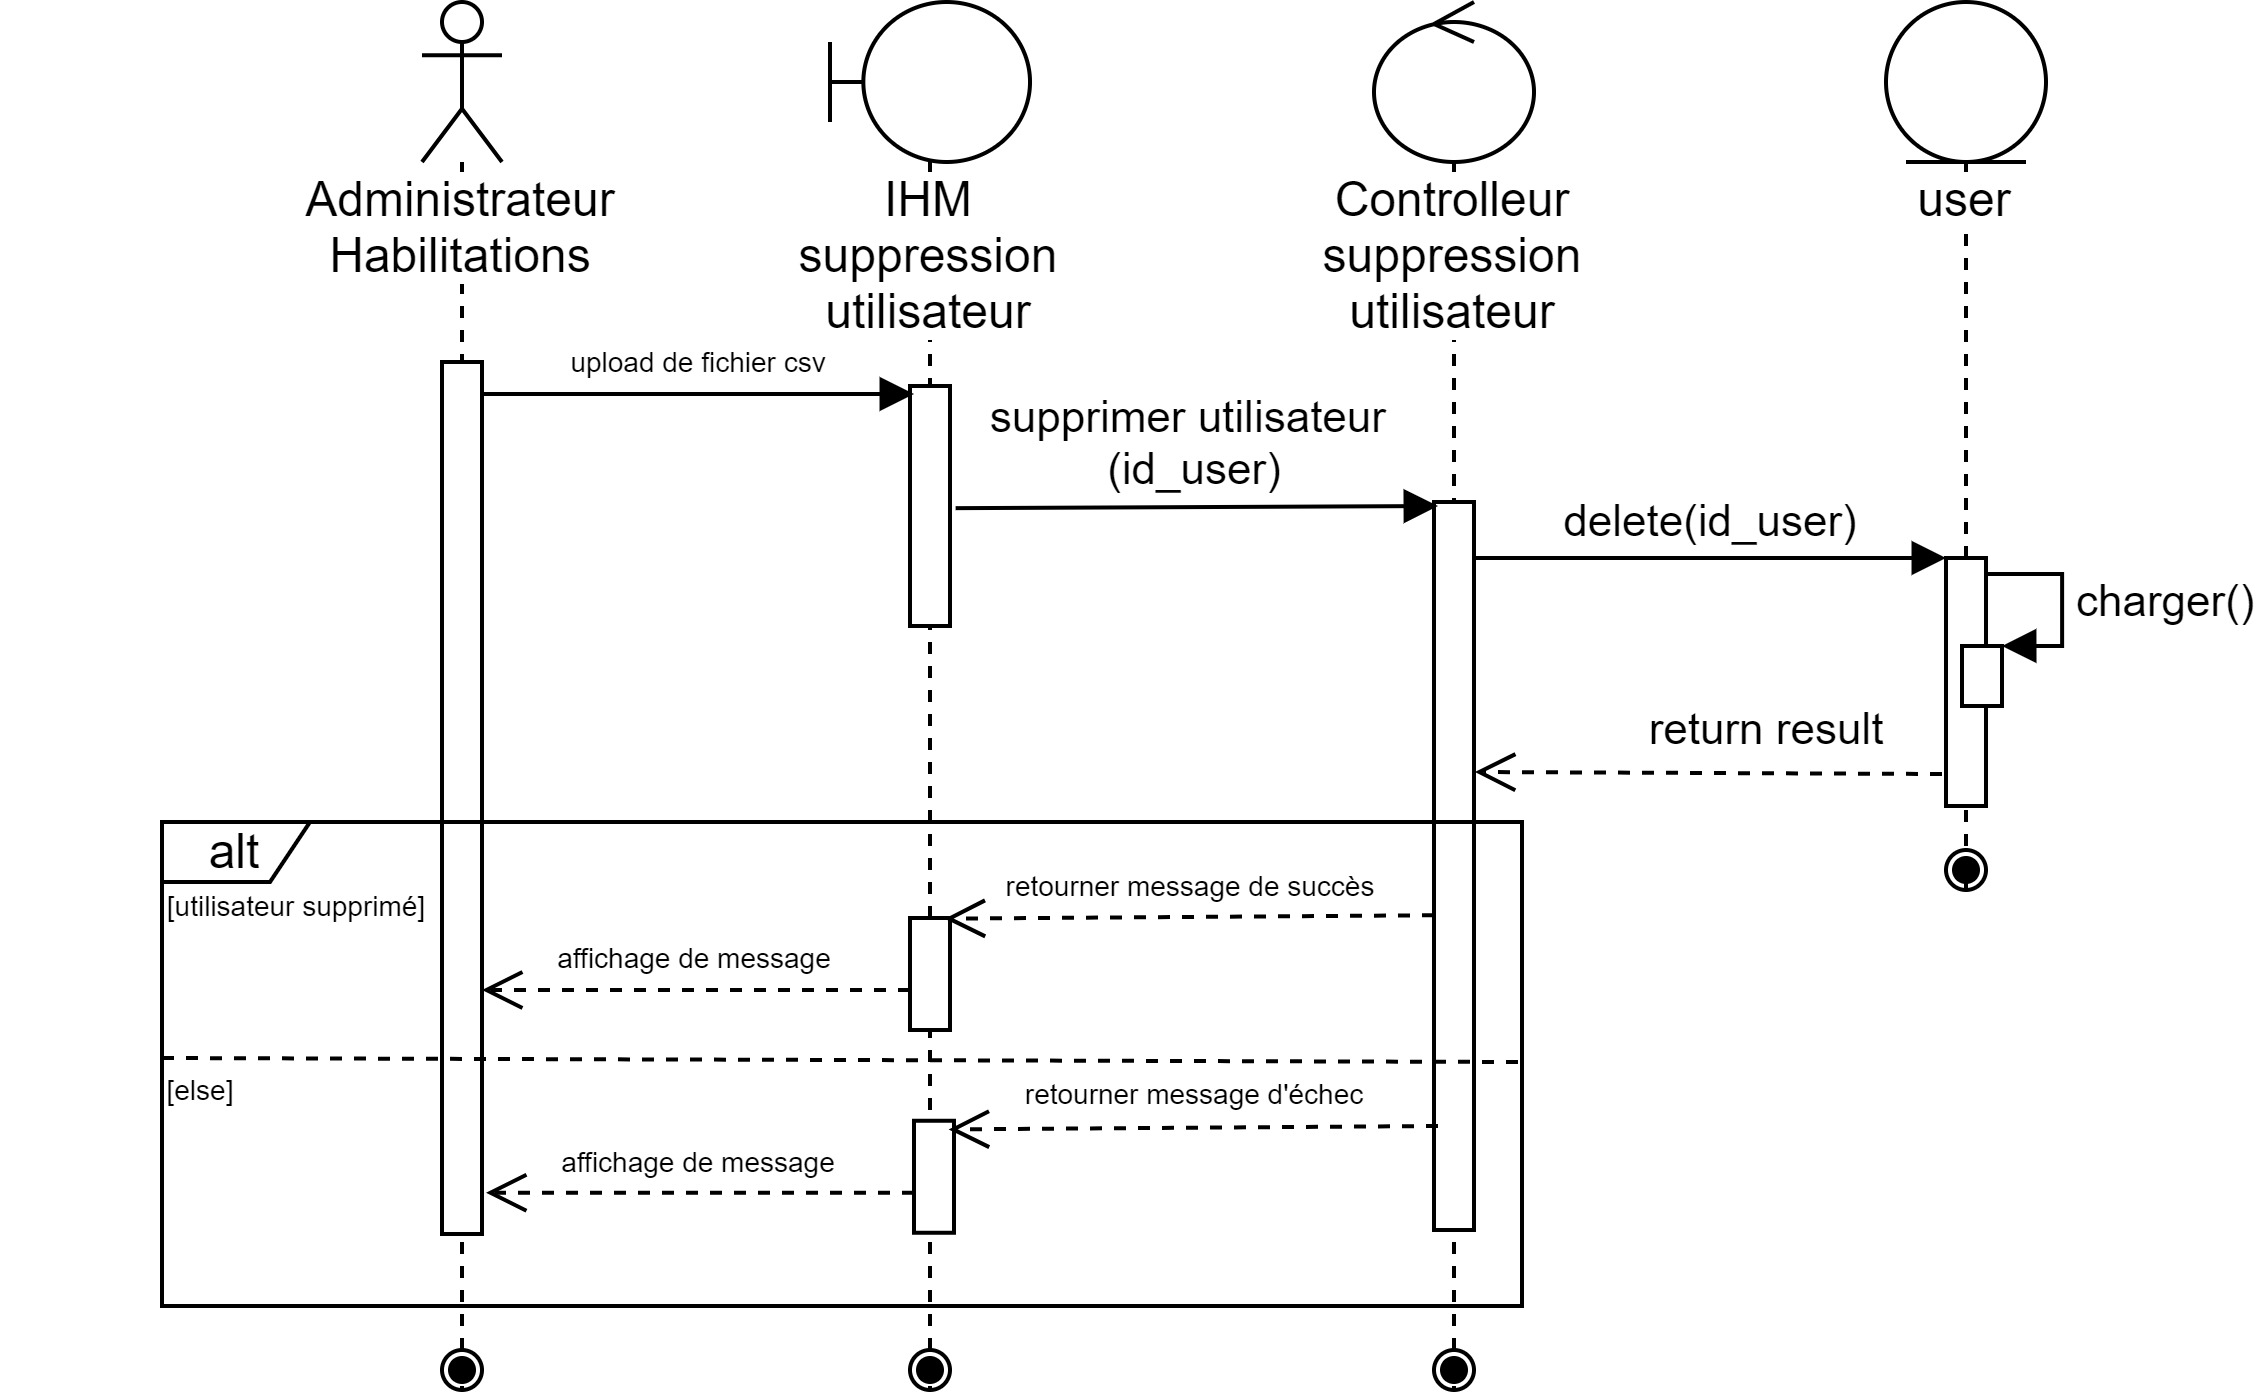
\includegraphics[width=0.75\linewidth]{img/conception/sequences/delete-obj}
	\caption[Diagramme de séquences objets de «Supprimer Utilisateur»]{Diagramme de séquences objets de «Supprimer Utilisateur»}
	\label{fig:delete-obj}
\end{figure}

\section[Réalisation]{Réalisation}
Dans cette sous-sections nous allons exposer les différentes interfaces réalisées dans le \\sprint 1. 
\subsection[Interfaces de gestion des utilisateurs]{Interfaces de gestion des utilisateurs}
les captures d'écran ci-dessous représentent les différentes IHM de gestion des utilisateurs.
\begin{itemize}
	\item Consultation des utilisateurs \& recherche
	\begin{figure}[H]
		\centering
		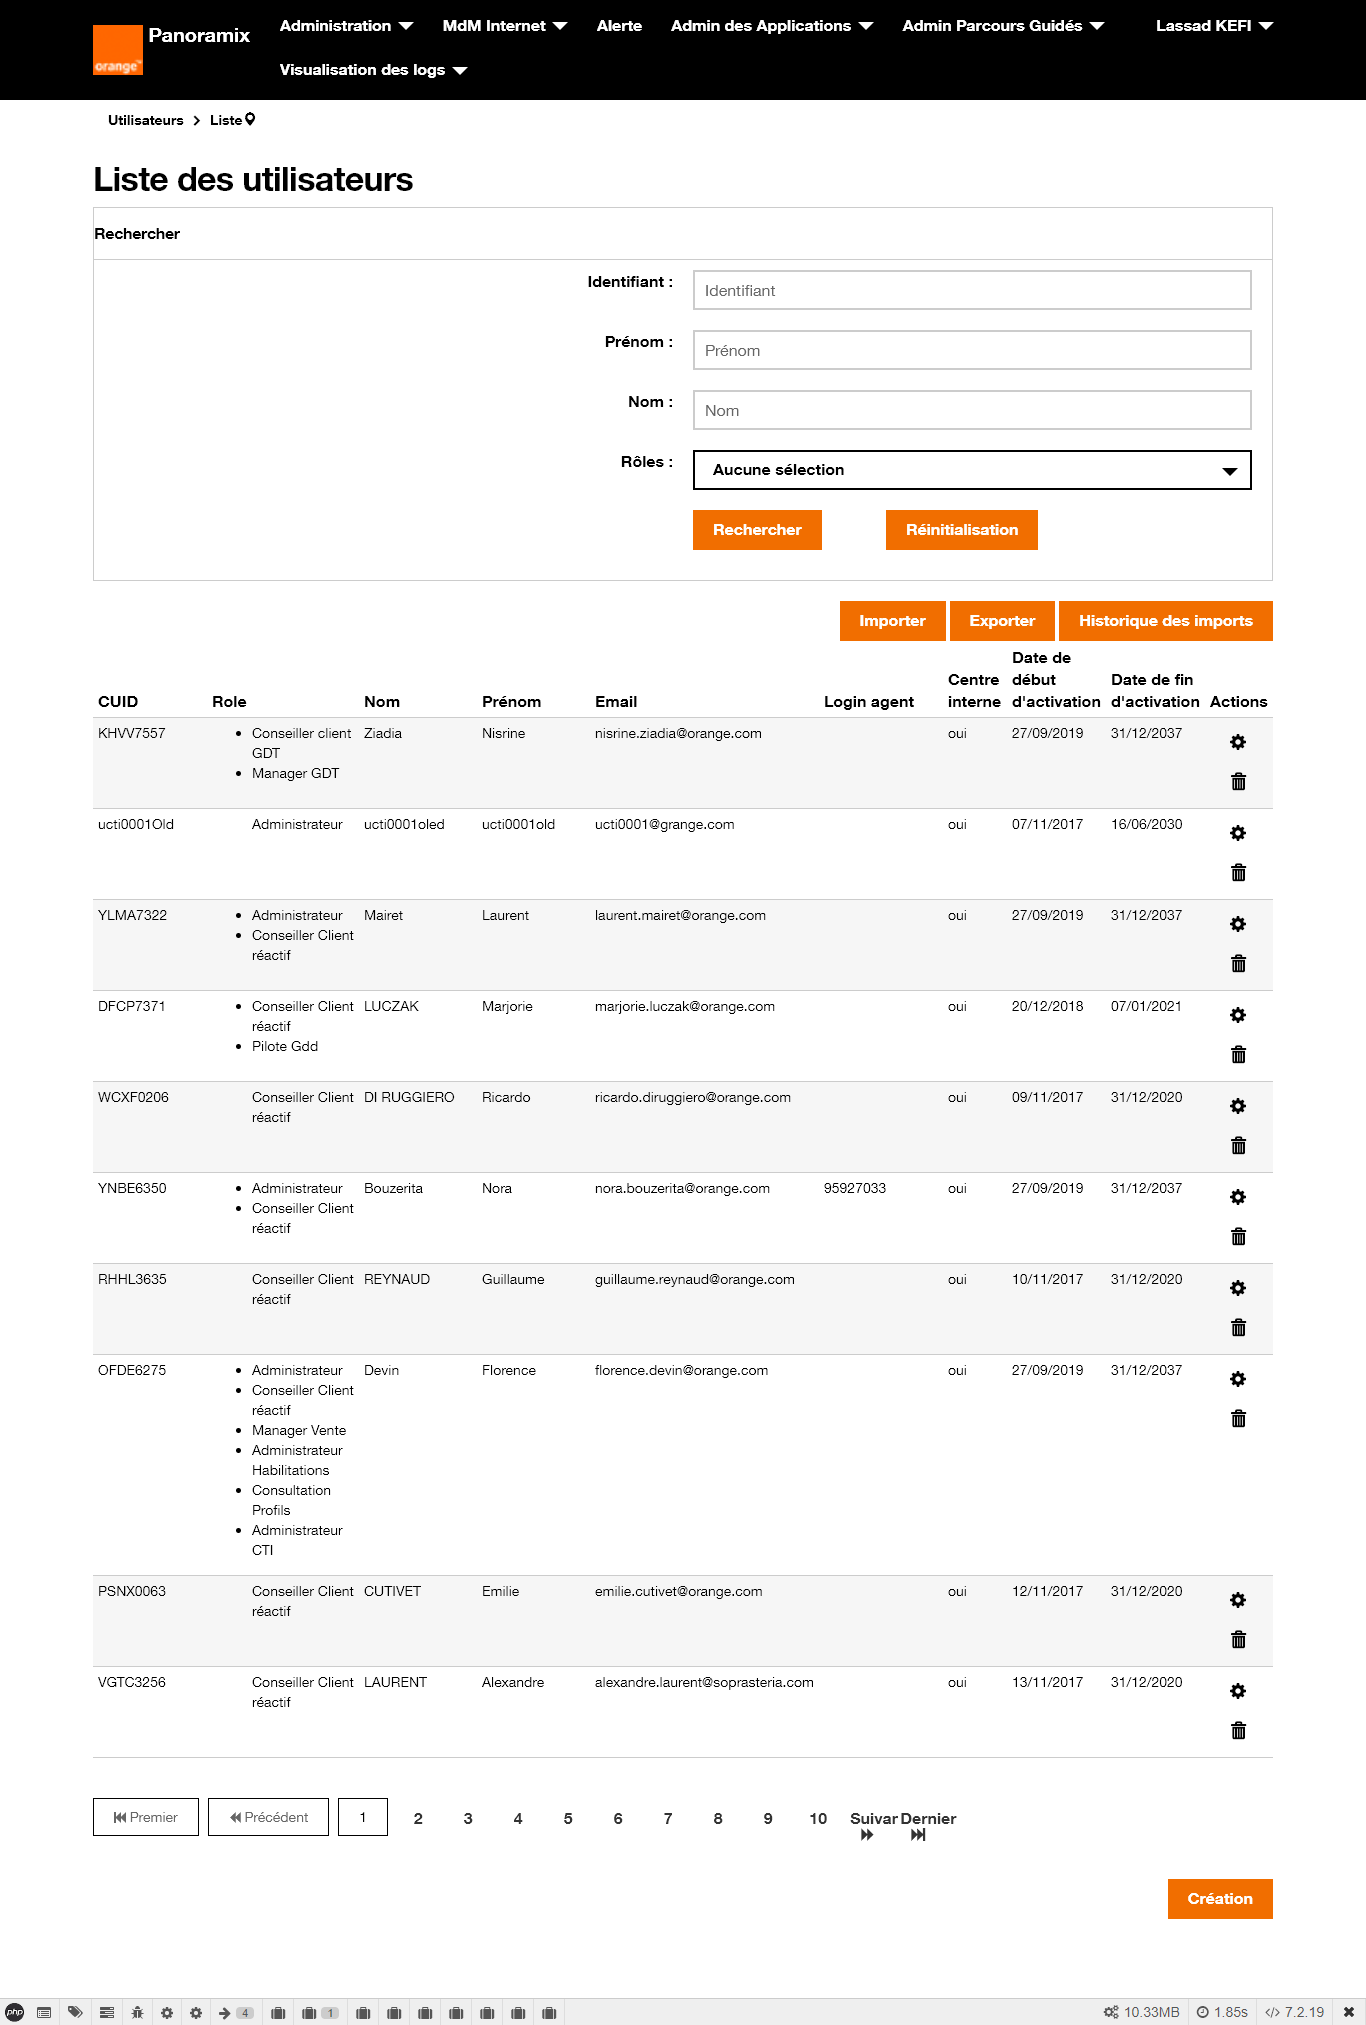
\includegraphics[width=0.7\linewidth]{img/screenshots/users/consultation}
		\caption[Interface consultation des utilisateurs et recherche]{Interface consultation des utilisateurs et recherche}
		\label{fig:consultation-user}
	\end{figure}
	
	\item Voir un utilisateur
	\begin{figure}[H]
		\centering
		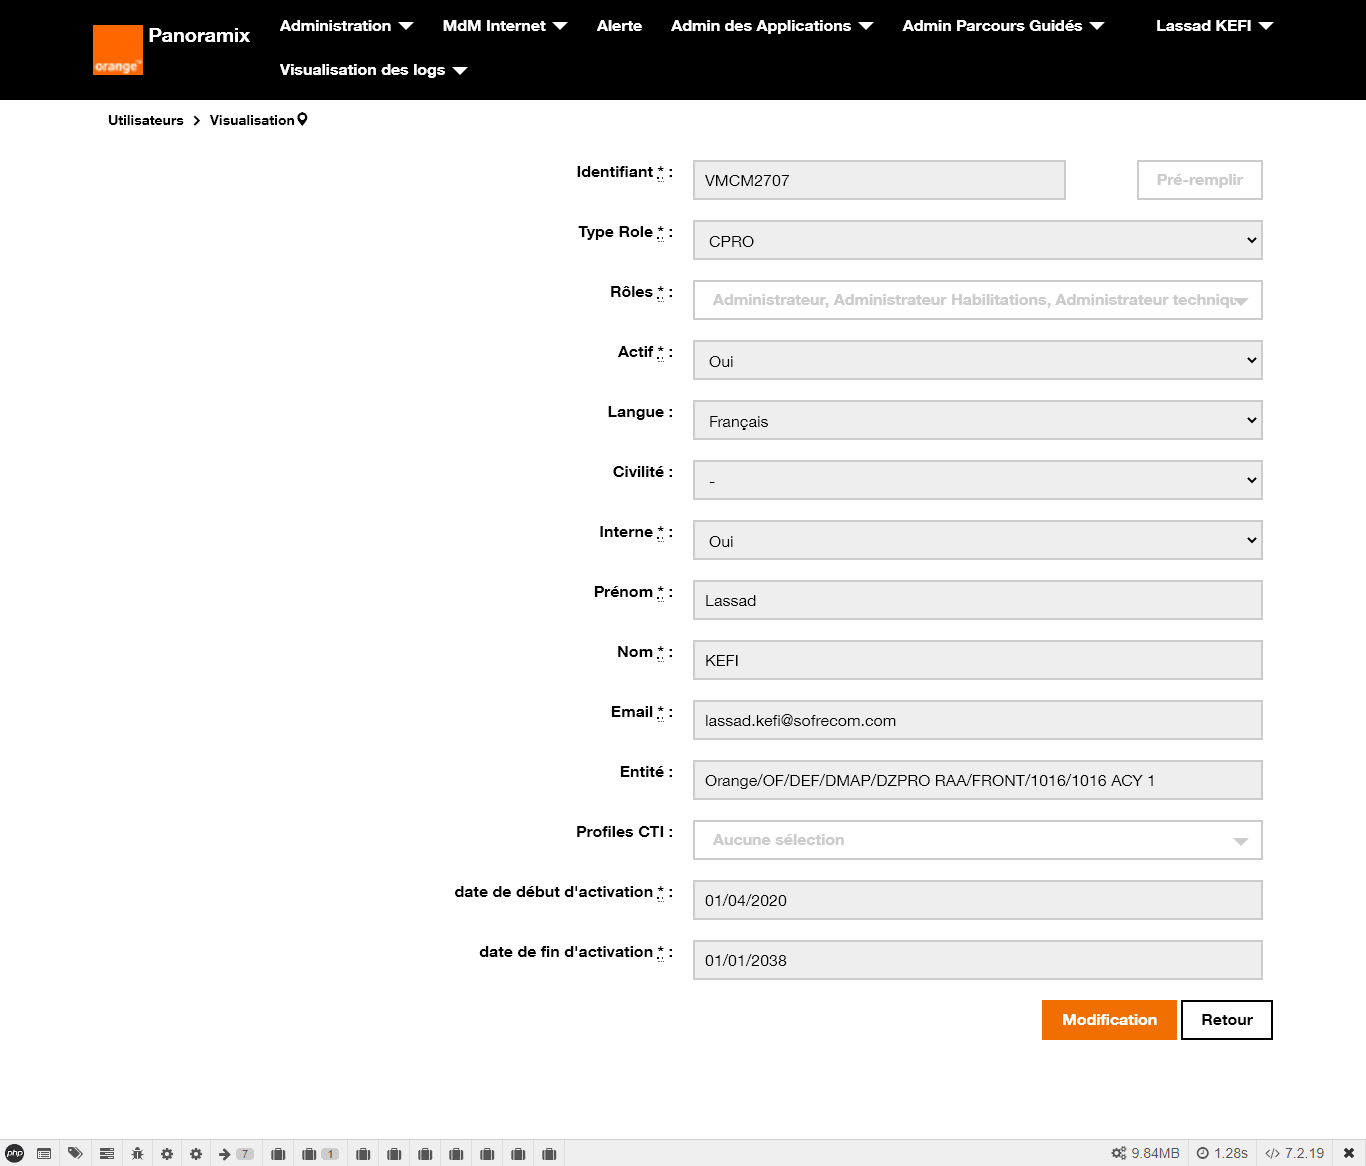
\includegraphics[width=0.65\linewidth]{img/screenshots/users/view}
		\caption[Interface voir utilisateur]{Interface voir utilisateur}
		\label{fig:view-user}
	\end{figure}

	\item Modifier ou créer utilisateur
	\begin{figure}[H]
		\centering
		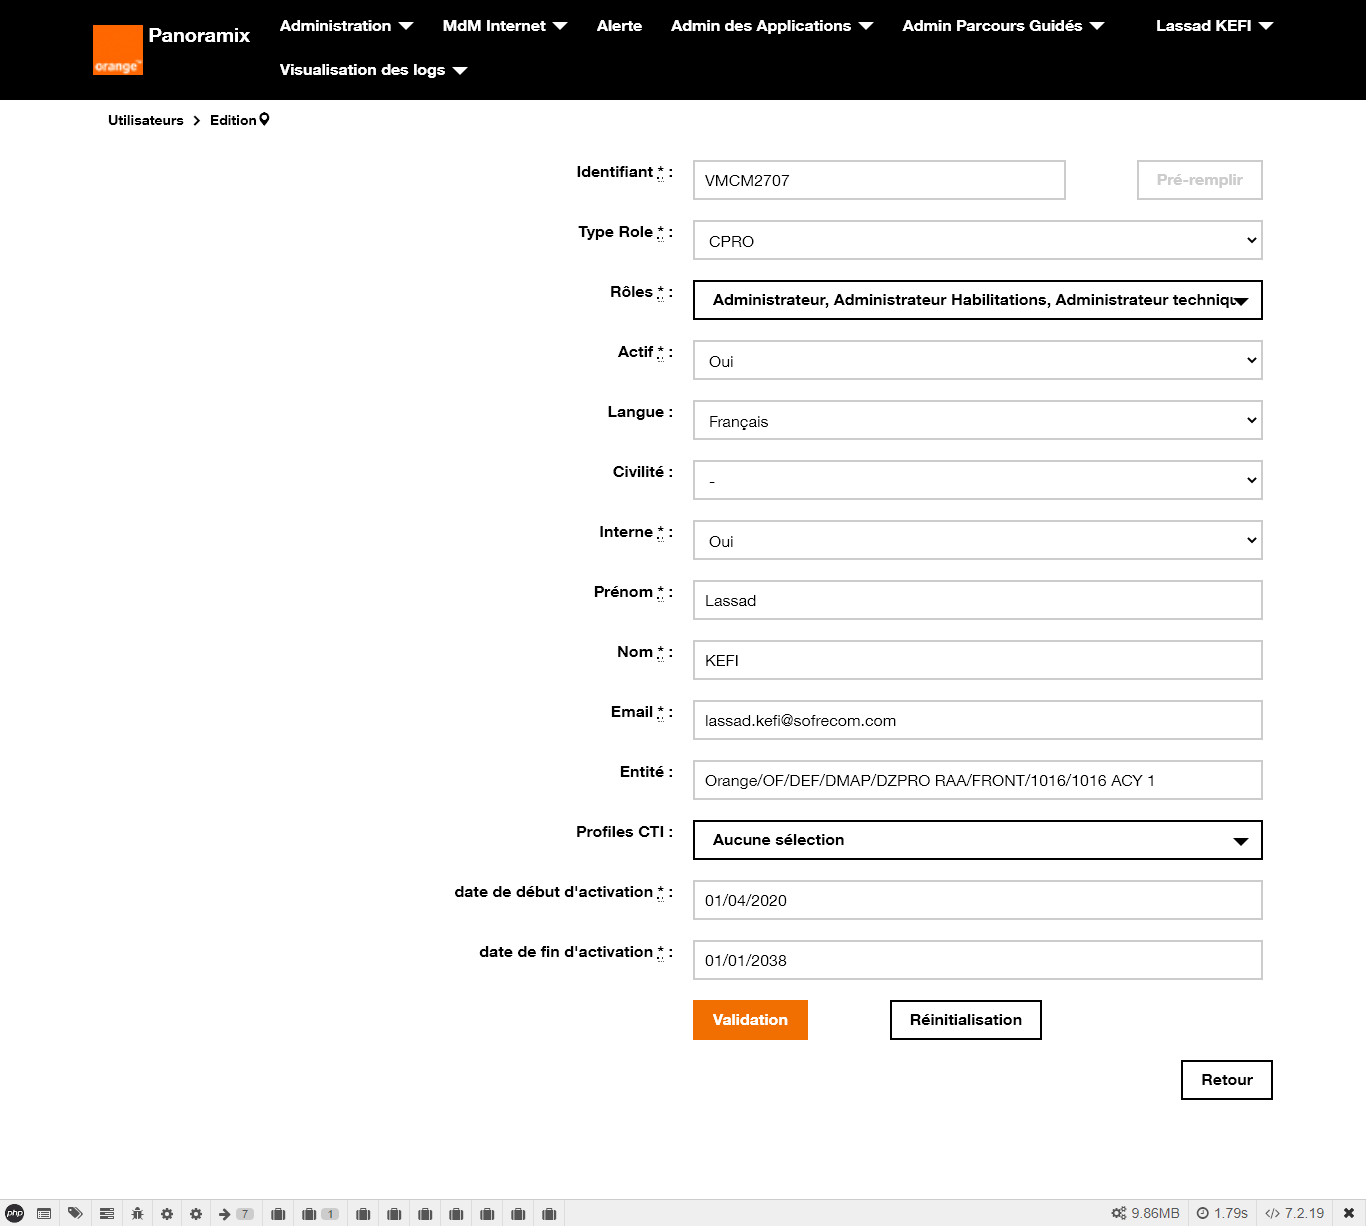
\includegraphics[width=0.65\linewidth]{img/screenshots/users/modif}
		\caption[Interface modifier ou créer utilisateur]{Interface modifier ou créer utilisateur}
		\label{fig:modif-user}
	\end{figure}
	\newpage
	\item Supprimer utilisateur
	\begin{figure}[H]
		\centering
		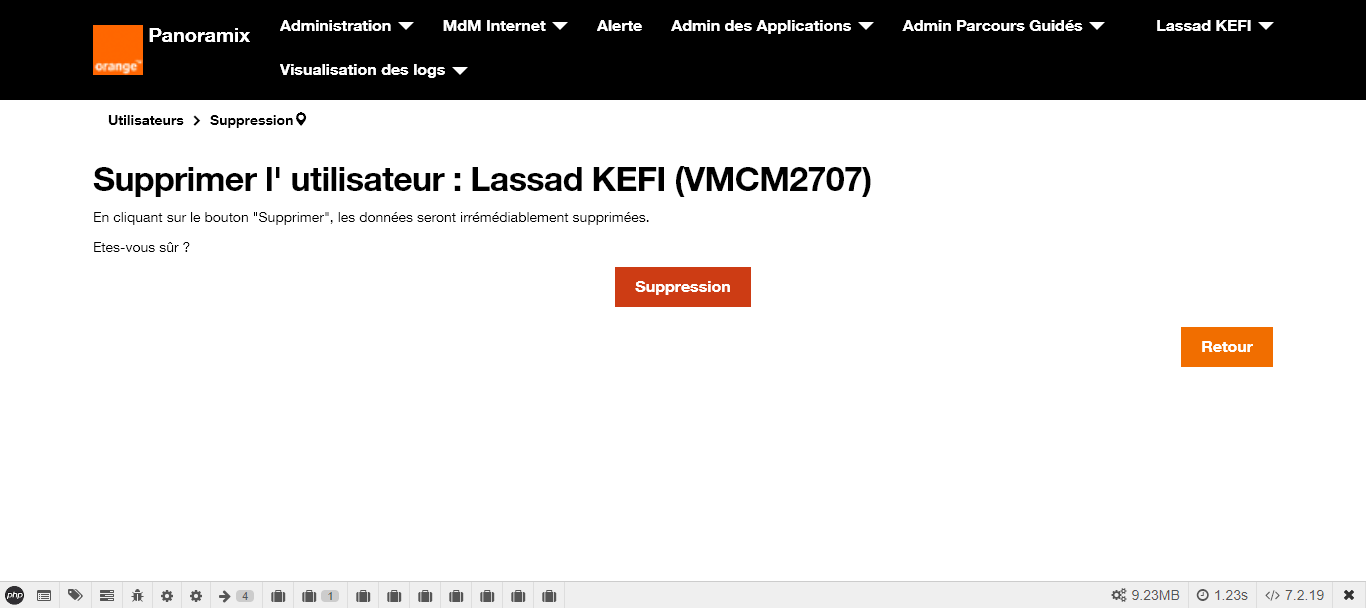
\includegraphics[width=0.65\linewidth]{img/screenshots/users/delete}
		\caption[Interface supprimer utilisateur]{Interface supprimer utilisateur}
		\label{fig:delete-user-ihm}
	\end{figure}

	\item Importer utilisateurs
	\begin{figure}[H]
		\centering
		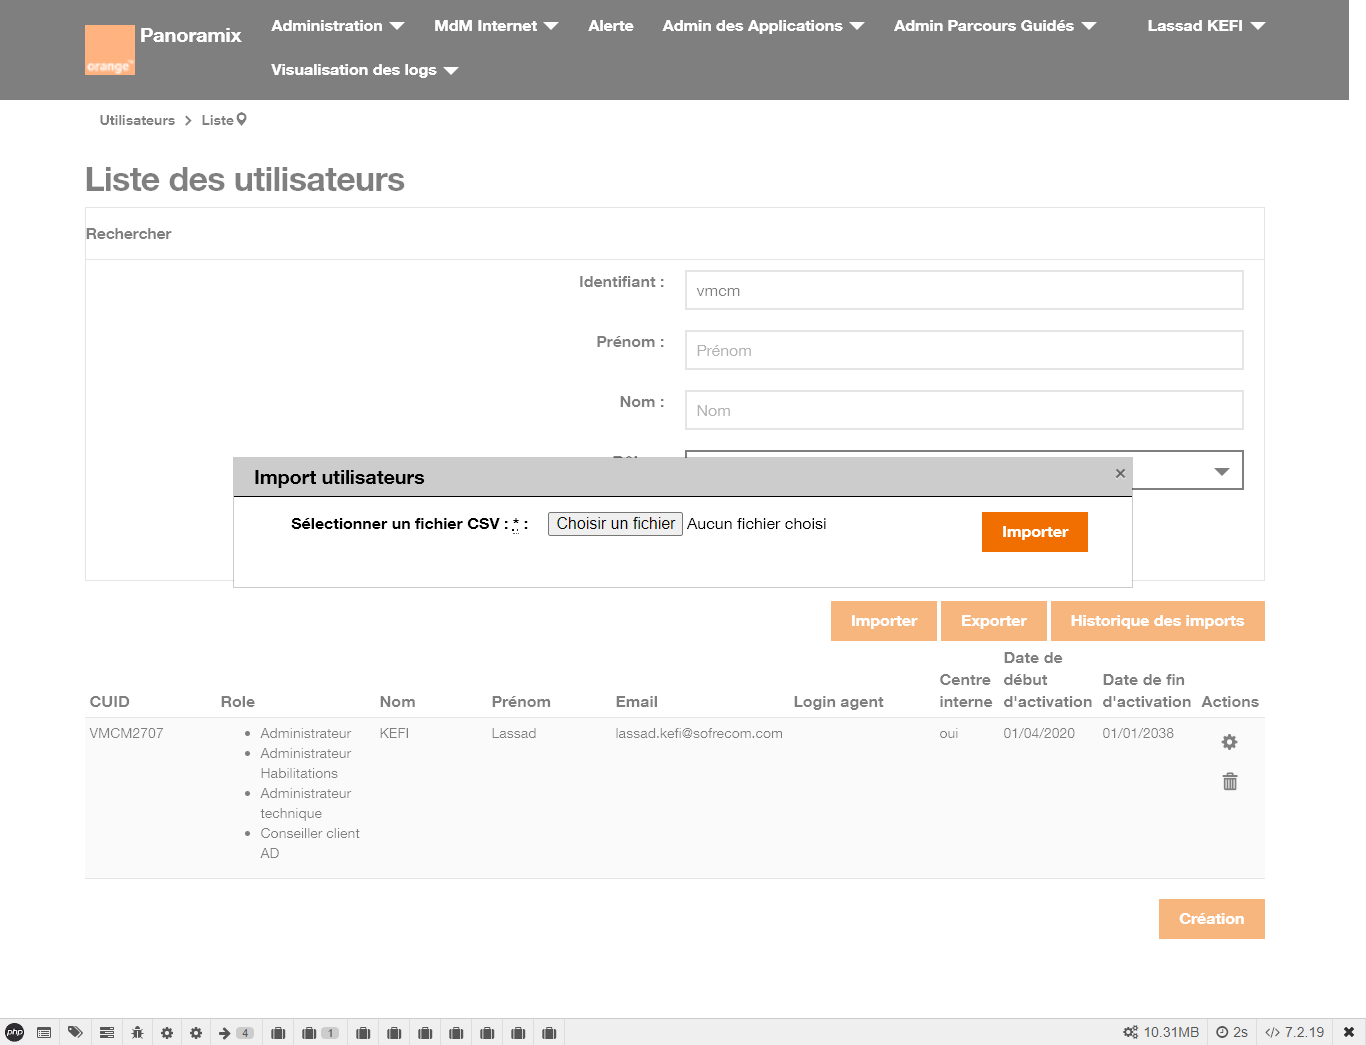
\includegraphics[width=0.65\linewidth]{img/screenshots/users/import}
		\caption[Interface importer utilisateurs]{Interface importer utilisateurs}
		\label{fig:import-user-ihm}
	\end{figure}

	\item Résultat d'exportation des utilisateurs
	\begin{figure}[H]
		\centering
		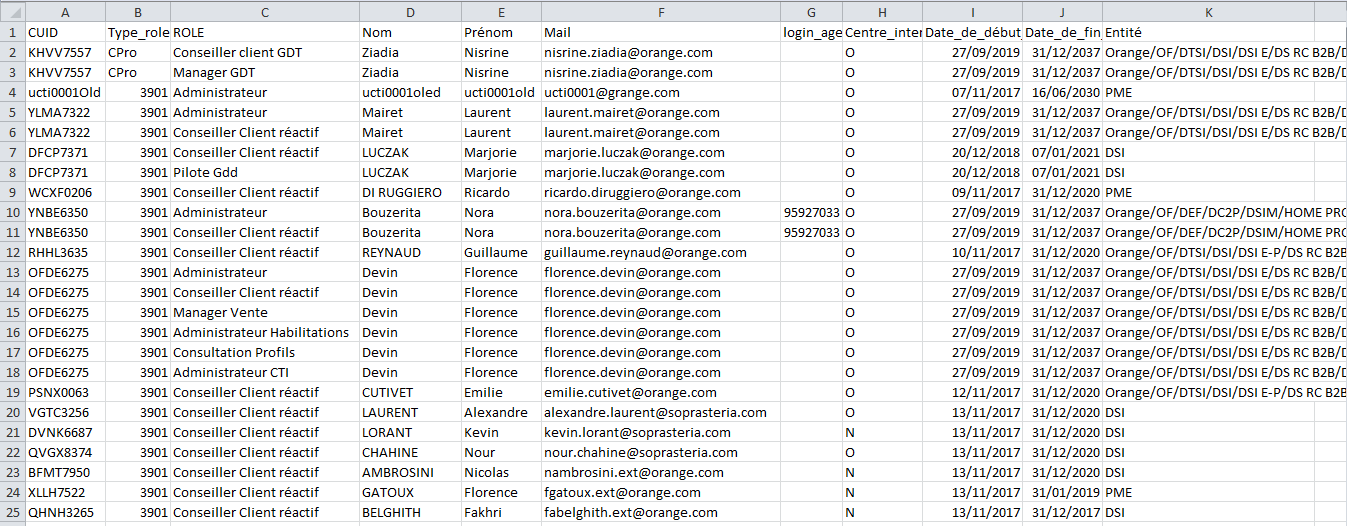
\includegraphics[width=0.65\linewidth]{img/screenshots/users/export}
		\caption[Interface résultat d'exportation des utilisateurs]{Interface résultat d'exportation des utilisateurs}
		\label{fig:export-user-ihm}
	\end{figure}
\end{itemize}

\subsection{Interfaces de gestion des rôles}
les captures d'écran ci-dessous représentent les différentes IHM de gestion des rôles.
\begin{itemize}
	\item Consultation des rôles et recherche
	\begin{figure}[H]
		\centering
		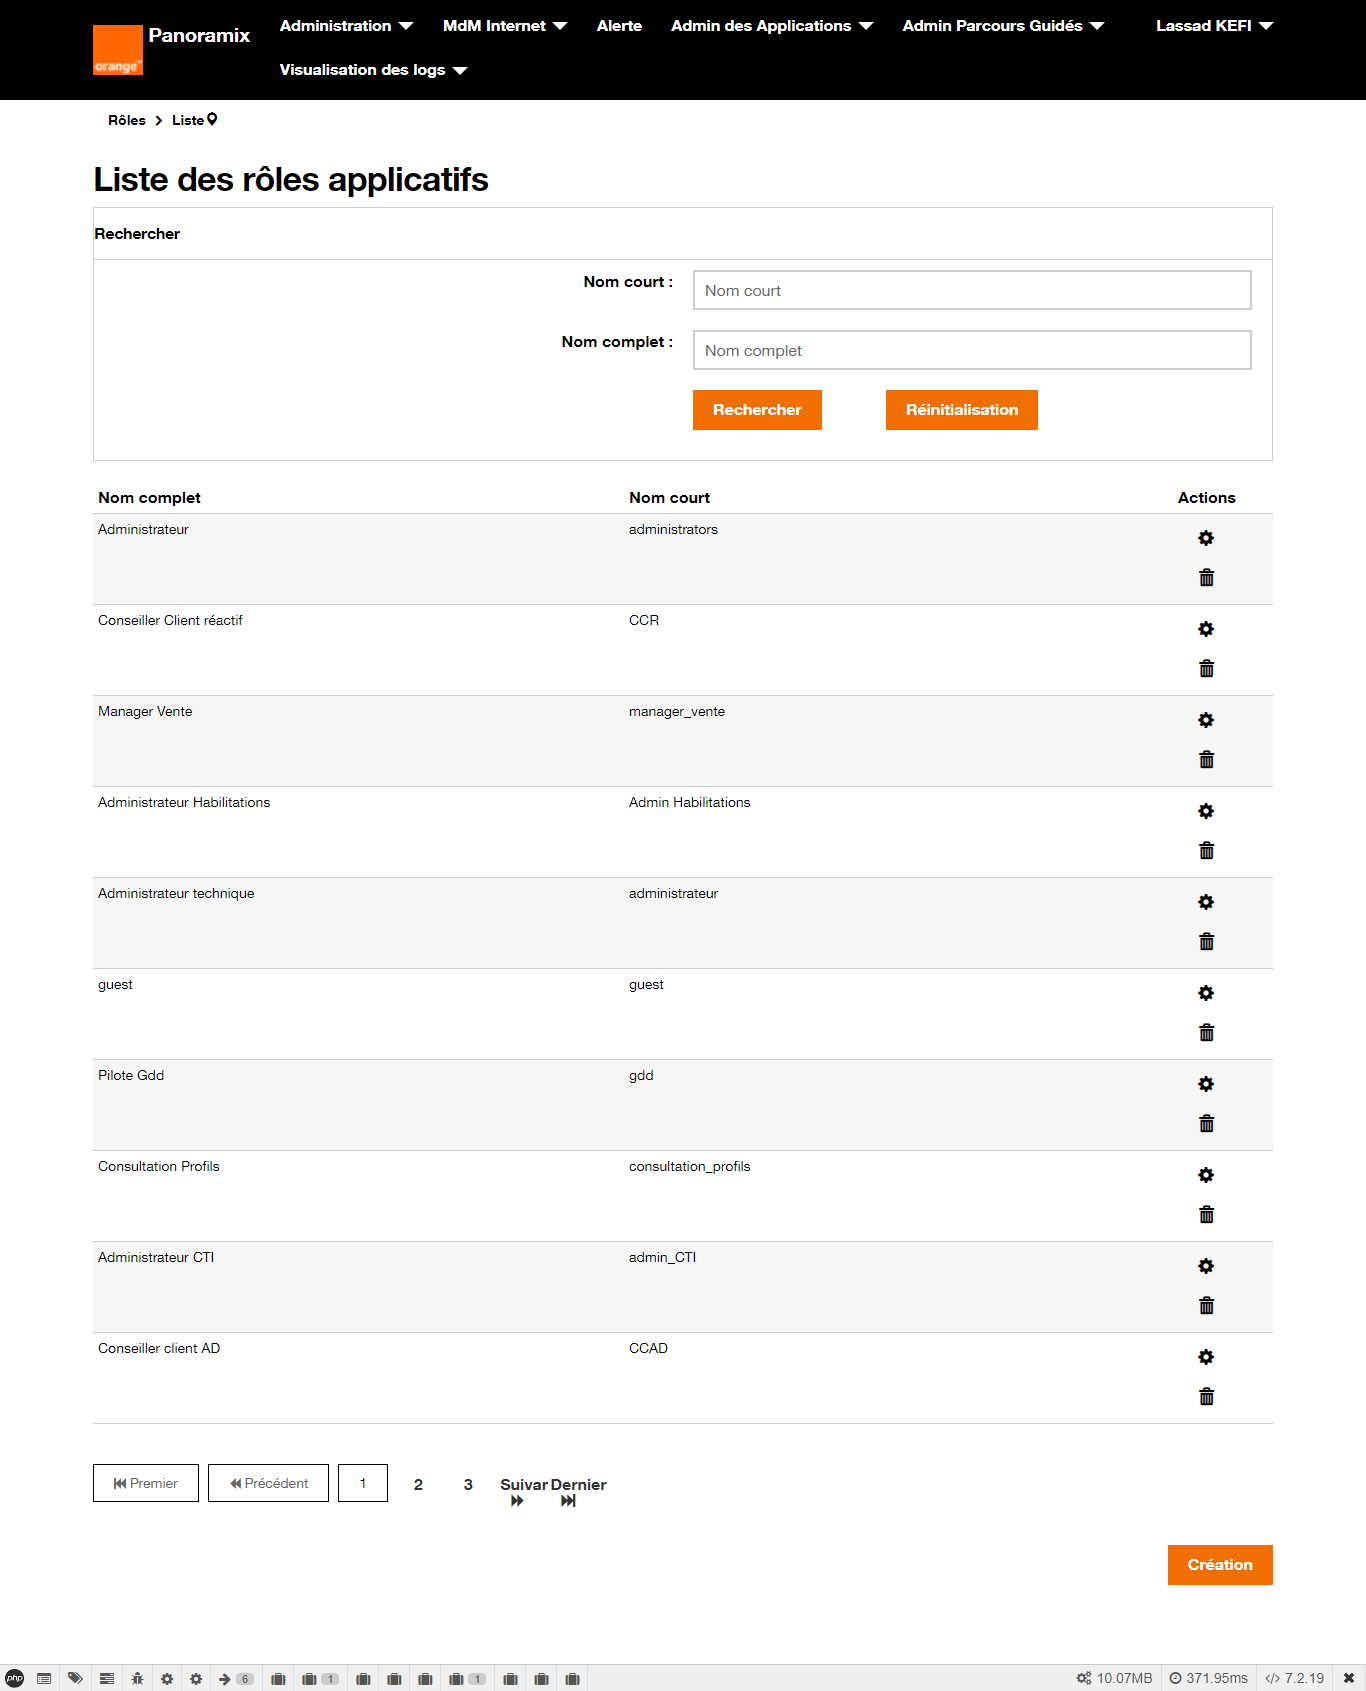
\includegraphics[width=0.6\linewidth]{img/screenshots/roles/index}
		\caption[Interface consultation des rôles]{Interface consultation des rôles et recherche}
		\label{fig:index-roles}
	\end{figure}
	
	\item Voir un rôle
	\begin{figure}[H]
		\centering
		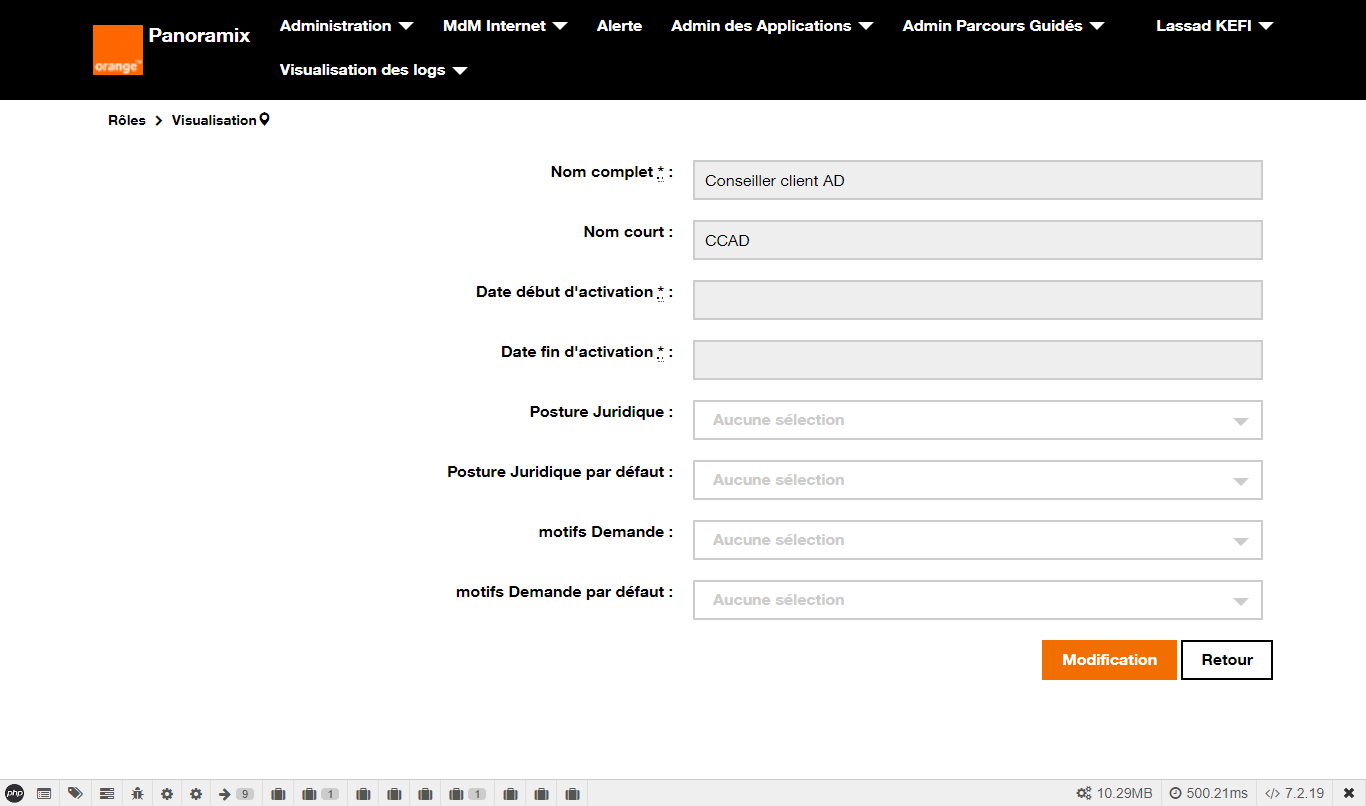
\includegraphics[width=0.6\linewidth]{img/screenshots/roles/view}
		\caption[Interface voir un rôle]{Interface voir un rôle}
		\label{fig:view-role}
	\end{figure}

	\item Modifier ou créer un rôle
	\begin{figure}[H]
		\centering
		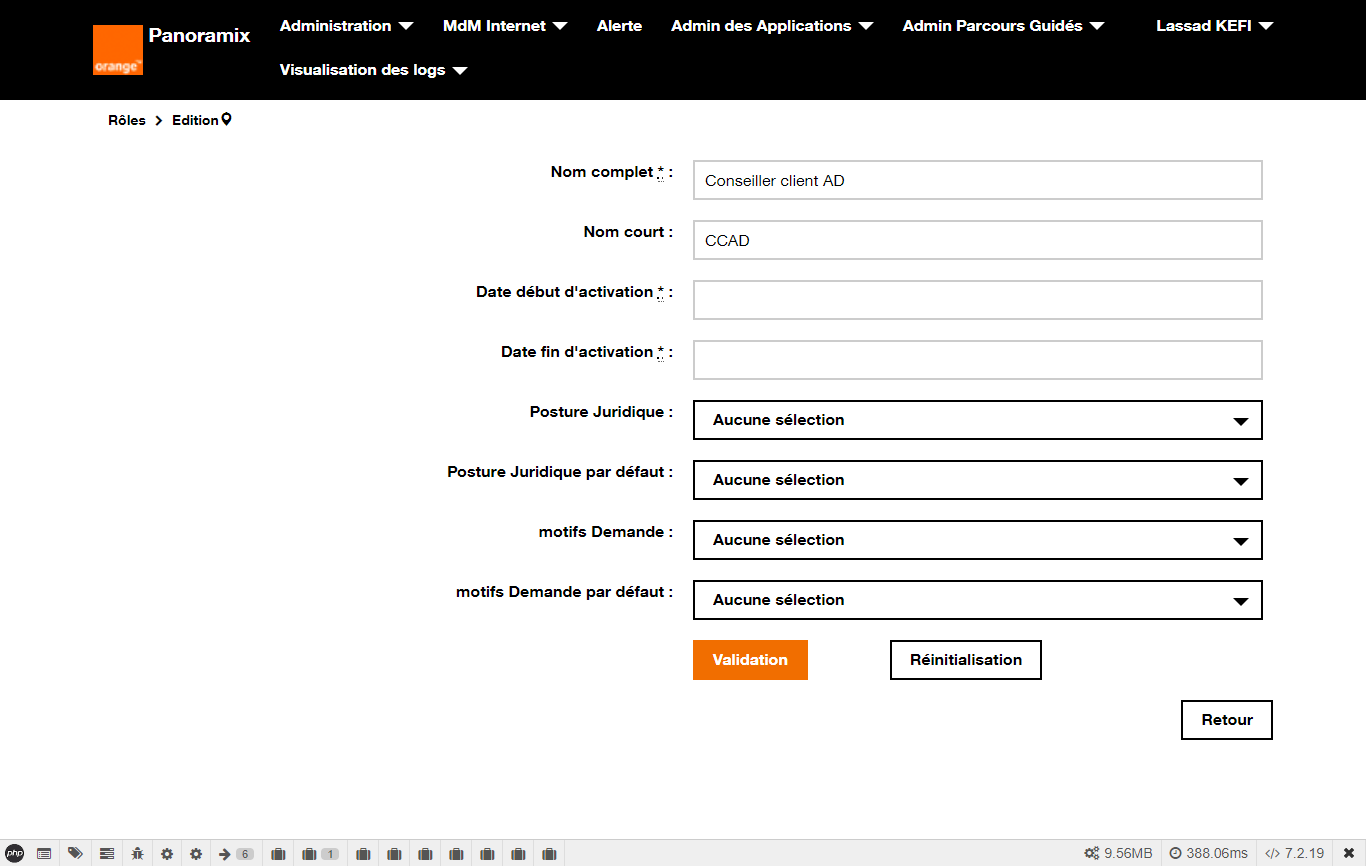
\includegraphics[width=0.7\linewidth]{img/screenshots/roles/edit}
		\caption[Interface modifier ou créer un rôle]{Interface modifier ou créer un rôle}
		\label{fig:modif-role}
	\end{figure}

	\item Supprimer un rôle
	\begin{figure}[H]
		\centering
		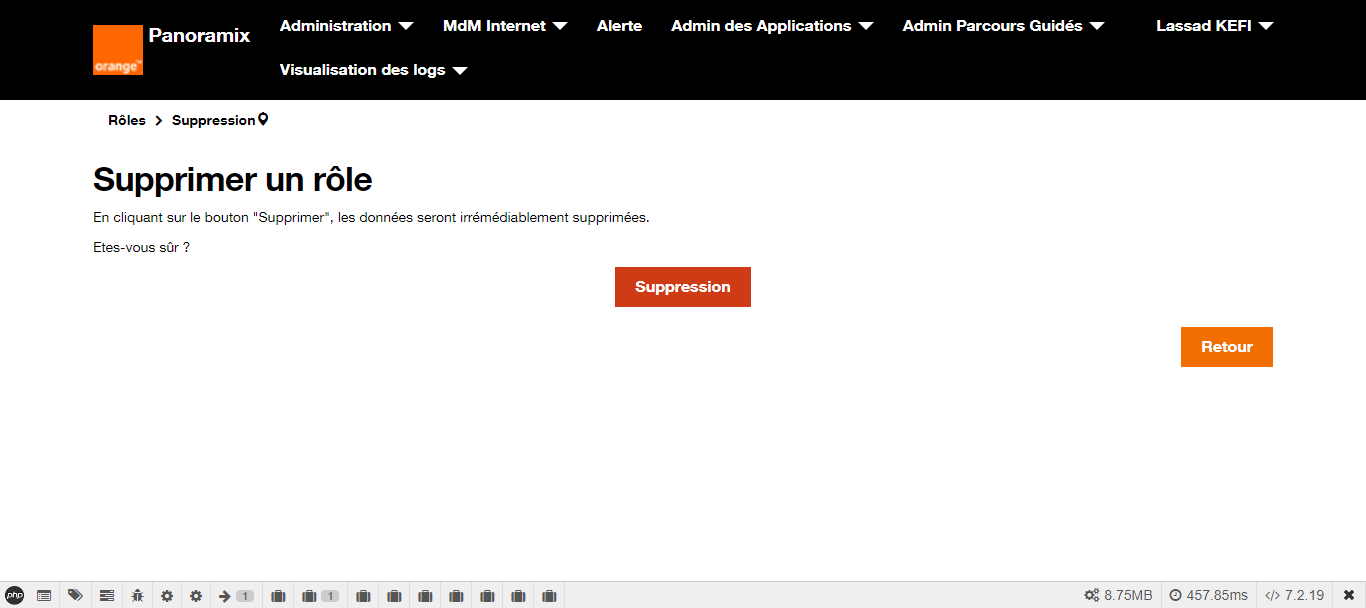
\includegraphics[width=0.7\linewidth]{img/screenshots/roles/delete}
		\caption[Interface sSupprimer un rôle]{Interface supprimer un rôle}
		\label{fig:delete-role}
	\end{figure}
\end{itemize}

\subsection{Interfaces de gestion des types de rôles}
les captures d'écran ci-dessous représentent les différentes IHM de gestion des types des rôles.
\newpage
\begin{itemize}
	\item Consultation des types de rôles et recherche
	\begin{figure}[H]
		\centering
		\includegraphics[width=0.7\linewidth]{"img/screenshots/type roles/index"}
		\caption[Interface consultation de types des rôles et recherche]{Interface consultation de types des rôles et recherche}
		\label{fig:index-tr}
	\end{figure}

	\item Voir les types d'un rôle 
	\begin{figure}[H]
		\centering
		\includegraphics[width=0.7\linewidth]{"img/screenshots/type roles/view"}
		\caption[Interface voir les types d'un rôle]{Interface voir les types d'un rôle}
		\label{fig:view-tr}
	\end{figure}
	\newpage
	\item Donner ou modifier des type à un rôle
	\begin{figure}[H]
		\centering
		\includegraphics[width=0.5\linewidth]{"img/screenshots/type roles/update"}
		\caption[Interface donner des type à un rôle]{Interface donner des type à un rôle}
		\label{fig:create-tr}
	\end{figure}
	
	\item Supprimer les type d'un rôle 
	\begin{figure}[H]
		\centering
		\includegraphics[width=0.5\linewidth]{"img/screenshots/type roles/delete"}
		\caption[Interface supprimer les type d'un rôle]{Interface supprimer les type d'un rôle}
		\label{fig:delete-tr}
	\end{figure}
\end{itemize}
\subsection{Interfaces de gestion des activations des rôles attribués à un utilisateurs}
les captures d'écran ci-dessous représentent les différentes IHM de des activations des rôles attribués à un utilisateurs.
\begin{itemize}
	\item Consultation des activations et recherche
	\begin{figure}[H]
		\centering
		\includegraphics[width=0.5\linewidth]{"img/screenshots/activation des roles/index"}
		\caption[Interface consultation des activations des rôles aux utilisateurs]{Interface consultation des activations des rôles aux utilisateurs}
		\label{fig:index-activation}
	\end{figure}
	
	\item Voir une activation de rôle d'un utilisateur
	\begin{figure}[H]
		\centering
		\includegraphics[width=0.7\linewidth]{"img/screenshots/activation des roles/view"}
		\caption[Interface voir une activation de rôle à un utilisateur]{Interface voir une activation de rôle à un utilisateur}
		\label{fig:view-activation}
	\end{figure}

	\item Activer/désactiver un rôle d'un utilisateurs
	\begin{figure}[H]
		\centering
		\includegraphics[width=0.7\linewidth]{"img/screenshots/activation des roles/edit"}
		\caption[Interface activer/désactiver un rôle d'un utilisateurs]{Interface activer/désactiver un rôle d'un utilisateurs}
		\label{fig:view-activation}
	\end{figure}
\end{itemize}

\section*{Conclusion}
Au cours de ce chapitre, nous avons réalisé le deuxième sprint qui permet de développer le module «Gestion des utilisateurs » et le module «Gestion des rôles» en rédigeant sa conception et donc la “release 1” est terminée. Dans le chapitre suivant, nous entamons le développement du premier sprint de release 2. 
